\documentclass[10pt]{article}
\usepackage{fullpage,enumitem,amsmath,amssymb,graphicx,hyperref, subfig}
\hypersetup{
    colorlinks=true,
    linkcolor=blue,
    filecolor=magenta,      
    urlcolor=cyan,
}
\usepackage{array}


\begin{document}

\begin{center}
{\Large CS224N Winter 2016 Homework 4 Milestone}
\begin{tabular}{rl}
SUNet ID: & [sijunhe, jiajuns, ming1993] \\
Name: & [Sijun He, Jiajun Sun, Mingxiang Chen] \\
\end{tabular}
\end{center}

By turning in this assignment, I agree by the Stanford honor code and declare
that all of this is my own work.
\section*{Finished}
\begin{enumerate}[label=(\alph*)]
\item Explored the dataset and the distribution of the length of context paragraphs and questions
\begin{figure}[ht]
\centering
    \subfloat{{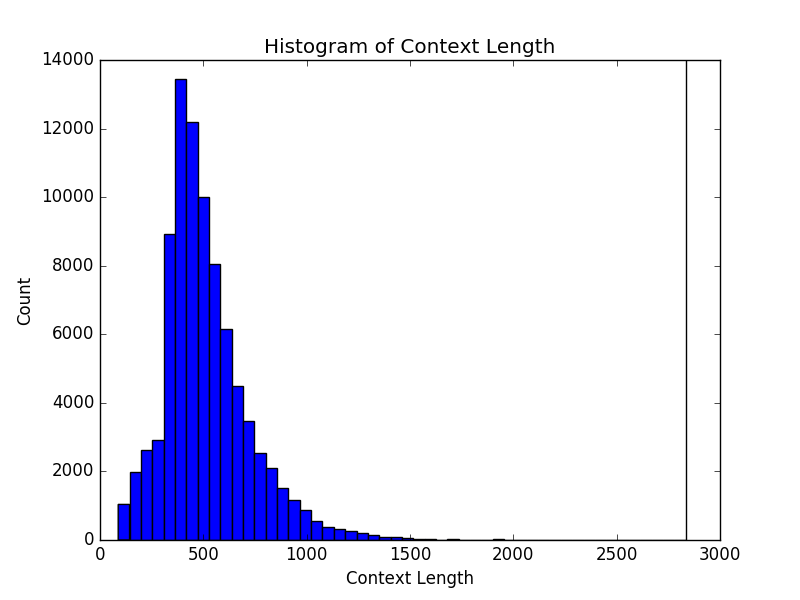
\includegraphics[scale=0.37]{context_hist.png} }}
    \qquad
    \subfloat{{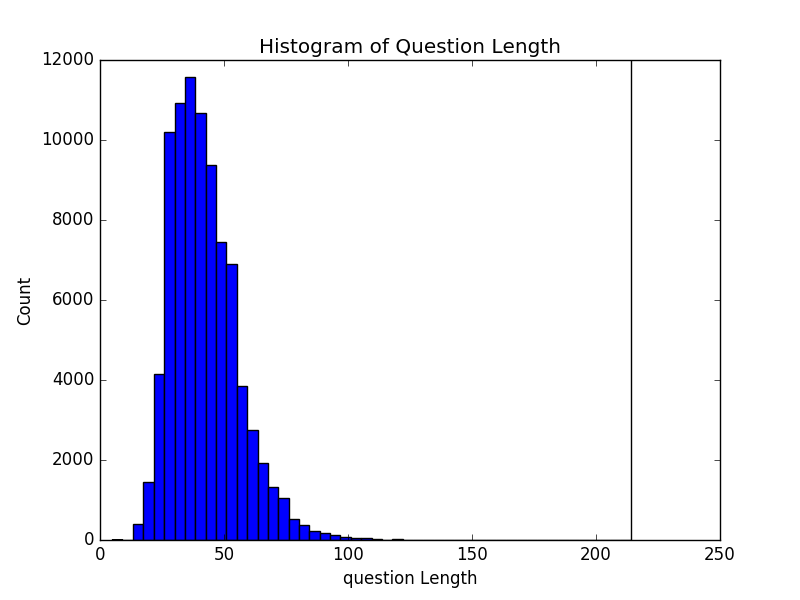
\includegraphics[scale=0.37]{question_hist.png} }}
\end{figure}
\item Various utility functions that load, preprocess(padding \& formatting for Tensorflow) and mini-batch the data.
\item configuring the GPU environment and download the dataset on Azure
\item Minimal model, with the purpose of setting up the architecture
\begin{enumerate}[label=(\roman*)]
\item LSTM to encode context into hidden vectors
\item Feed-Forward Neural Network as decoder for a 2-class classification
\item Model can be trained, though accuracy is extremely low due to not using question data :( and very imbalanced classification.
\end{enumerate}
\item A baseline model
\begin{enumerate}[label=(\roman*)]
\item BiLSTM to encode the context with all hidden states, BiLSTM to encode the question with the final hidden state
\item Word alignment layer with bilinear attention of question representation over the context representation 
\end{enumerate}
\end{enumerate}
\section*{In Progress}
\begin{enumerate}[label=(\alph*)]
\item Baseline model
\begin{enumerate}[label=(\roman*)]
\item LSTM and two separate Feed-Forward Neural Network to model $P(a_s|\text{context}, \text{question})$  and $P(a_e|\text{context}, \text{question})$, as described in \hyperlink{https://arxiv.org/abs/1612.04211}{Multi-Perspective Matching}
\end{enumerate}
\end{enumerate}
\end{document}

